% Options for packages loaded elsewhere
\PassOptionsToPackage{unicode}{hyperref}
\PassOptionsToPackage{hyphens}{url}
%
\documentclass[
]{article}
\usepackage{amsmath,amssymb}
\usepackage{iftex}
\ifPDFTeX
  \usepackage[T1]{fontenc}
  \usepackage[utf8]{inputenc}
  \usepackage{textcomp} % provide euro and other symbols
\else % if luatex or xetex
  \usepackage{unicode-math} % this also loads fontspec
  \defaultfontfeatures{Scale=MatchLowercase}
  \defaultfontfeatures[\rmfamily]{Ligatures=TeX,Scale=1}
\fi
\usepackage{lmodern}
\ifPDFTeX\else
  % xetex/luatex font selection
\fi
% Use upquote if available, for straight quotes in verbatim environments
\IfFileExists{upquote.sty}{\usepackage{upquote}}{}
\IfFileExists{microtype.sty}{% use microtype if available
  \usepackage[]{microtype}
  \UseMicrotypeSet[protrusion]{basicmath} % disable protrusion for tt fonts
}{}
\makeatletter
\@ifundefined{KOMAClassName}{% if non-KOMA class
  \IfFileExists{parskip.sty}{%
    \usepackage{parskip}
  }{% else
    \setlength{\parindent}{0pt}
    \setlength{\parskip}{6pt plus 2pt minus 1pt}}
}{% if KOMA class
  \KOMAoptions{parskip=half}}
\makeatother
\usepackage{xcolor}
\usepackage[margin=1in]{geometry}
\usepackage{color}
\usepackage{fancyvrb}
\newcommand{\VerbBar}{|}
\newcommand{\VERB}{\Verb[commandchars=\\\{\}]}
\DefineVerbatimEnvironment{Highlighting}{Verbatim}{commandchars=\\\{\}}
% Add ',fontsize=\small' for more characters per line
\usepackage{framed}
\definecolor{shadecolor}{RGB}{248,248,248}
\newenvironment{Shaded}{\begin{snugshade}}{\end{snugshade}}
\newcommand{\AlertTok}[1]{\textcolor[rgb]{0.94,0.16,0.16}{#1}}
\newcommand{\AnnotationTok}[1]{\textcolor[rgb]{0.56,0.35,0.01}{\textbf{\textit{#1}}}}
\newcommand{\AttributeTok}[1]{\textcolor[rgb]{0.13,0.29,0.53}{#1}}
\newcommand{\BaseNTok}[1]{\textcolor[rgb]{0.00,0.00,0.81}{#1}}
\newcommand{\BuiltInTok}[1]{#1}
\newcommand{\CharTok}[1]{\textcolor[rgb]{0.31,0.60,0.02}{#1}}
\newcommand{\CommentTok}[1]{\textcolor[rgb]{0.56,0.35,0.01}{\textit{#1}}}
\newcommand{\CommentVarTok}[1]{\textcolor[rgb]{0.56,0.35,0.01}{\textbf{\textit{#1}}}}
\newcommand{\ConstantTok}[1]{\textcolor[rgb]{0.56,0.35,0.01}{#1}}
\newcommand{\ControlFlowTok}[1]{\textcolor[rgb]{0.13,0.29,0.53}{\textbf{#1}}}
\newcommand{\DataTypeTok}[1]{\textcolor[rgb]{0.13,0.29,0.53}{#1}}
\newcommand{\DecValTok}[1]{\textcolor[rgb]{0.00,0.00,0.81}{#1}}
\newcommand{\DocumentationTok}[1]{\textcolor[rgb]{0.56,0.35,0.01}{\textbf{\textit{#1}}}}
\newcommand{\ErrorTok}[1]{\textcolor[rgb]{0.64,0.00,0.00}{\textbf{#1}}}
\newcommand{\ExtensionTok}[1]{#1}
\newcommand{\FloatTok}[1]{\textcolor[rgb]{0.00,0.00,0.81}{#1}}
\newcommand{\FunctionTok}[1]{\textcolor[rgb]{0.13,0.29,0.53}{\textbf{#1}}}
\newcommand{\ImportTok}[1]{#1}
\newcommand{\InformationTok}[1]{\textcolor[rgb]{0.56,0.35,0.01}{\textbf{\textit{#1}}}}
\newcommand{\KeywordTok}[1]{\textcolor[rgb]{0.13,0.29,0.53}{\textbf{#1}}}
\newcommand{\NormalTok}[1]{#1}
\newcommand{\OperatorTok}[1]{\textcolor[rgb]{0.81,0.36,0.00}{\textbf{#1}}}
\newcommand{\OtherTok}[1]{\textcolor[rgb]{0.56,0.35,0.01}{#1}}
\newcommand{\PreprocessorTok}[1]{\textcolor[rgb]{0.56,0.35,0.01}{\textit{#1}}}
\newcommand{\RegionMarkerTok}[1]{#1}
\newcommand{\SpecialCharTok}[1]{\textcolor[rgb]{0.81,0.36,0.00}{\textbf{#1}}}
\newcommand{\SpecialStringTok}[1]{\textcolor[rgb]{0.31,0.60,0.02}{#1}}
\newcommand{\StringTok}[1]{\textcolor[rgb]{0.31,0.60,0.02}{#1}}
\newcommand{\VariableTok}[1]{\textcolor[rgb]{0.00,0.00,0.00}{#1}}
\newcommand{\VerbatimStringTok}[1]{\textcolor[rgb]{0.31,0.60,0.02}{#1}}
\newcommand{\WarningTok}[1]{\textcolor[rgb]{0.56,0.35,0.01}{\textbf{\textit{#1}}}}
\usepackage{graphicx}
\makeatletter
\def\maxwidth{\ifdim\Gin@nat@width>\linewidth\linewidth\else\Gin@nat@width\fi}
\def\maxheight{\ifdim\Gin@nat@height>\textheight\textheight\else\Gin@nat@height\fi}
\makeatother
% Scale images if necessary, so that they will not overflow the page
% margins by default, and it is still possible to overwrite the defaults
% using explicit options in \includegraphics[width, height, ...]{}
\setkeys{Gin}{width=\maxwidth,height=\maxheight,keepaspectratio}
% Set default figure placement to htbp
\makeatletter
\def\fps@figure{htbp}
\makeatother
\setlength{\emergencystretch}{3em} % prevent overfull lines
\providecommand{\tightlist}{%
  \setlength{\itemsep}{0pt}\setlength{\parskip}{0pt}}
\setcounter{secnumdepth}{-\maxdimen} % remove section numbering
\usepackage{booktabs}
\usepackage{longtable}
\usepackage{array}
\usepackage{multirow}
\usepackage{wrapfig}
\usepackage{float}
\usepackage{colortbl}
\usepackage{pdflscape}
\usepackage{tabu}
\usepackage{threeparttable}
\usepackage{threeparttablex}
\usepackage[normalem]{ulem}
\usepackage{makecell}
\usepackage{xcolor}
\usepackage{siunitx}

  \newcolumntype{d}{S[
    input-open-uncertainty=,
    input-close-uncertainty=,
    parse-numbers = false,
    table-align-text-pre=false,
    table-align-text-post=false
  ]}
  
\ifLuaTeX
  \usepackage{selnolig}  % disable illegal ligatures
\fi
\IfFileExists{bookmark.sty}{\usepackage{bookmark}}{\usepackage{hyperref}}
\IfFileExists{xurl.sty}{\usepackage{xurl}}{} % add URL line breaks if available
\urlstyle{same}
\hypersetup{
  pdftitle={ECO 530 - Fall 2023   Exercise 3},
  pdfauthor={Devan Arnold},
  hidelinks,
  pdfcreator={LaTeX via pandoc}}

\title{ECO 530 - Fall 2023 Exercise 3}
\author{Devan Arnold}
\date{Due: Oct 6, 2023}

\begin{document}
\maketitle

\DeclareMathOperator{\Lagr}{\mathcal{L}}
\DeclareMathOperator{\sumn}{\sum_{i=1}^n}
\DeclareMathOperator{\bh}{\hat{\beta}}
\DeclareMathOperator{\yh}{\hat{y}}
\DeclareMathOperator{\ybar}{\bar{y}}
\DeclareMathOperator{\xbar}{\bar{x}}
\usepackage{amsmath}

\hypertarget{instructions}{%
\section{Instructions}\label{instructions}}

Complete the exercises below using the Nicaragua Rural Business
Development Data (NicaRBD.RData). Be sure to show all of your work. For
this assignment, you can submit:

\begin{itemize}
\item
  A PDF containing your written answers, tables, and figures along with
  the R script that generates them
\item
  A PDF document containing your written answers with the R code
  embedded in the document.
\end{itemize}

\hfill\break

\hfill\break

\hypertarget{q1}{%
\section{Q1}\label{q1}}

\textbf{In this assignment, we are going to explore the relationship
between technical efficiency in maize production (\texttt{te\_maize})
and food expenditure (\texttt{food.expend}). We will also consider the
relationships between access to credit (\texttt{couldgetloan}), holding
formal land title (\texttt{writtentitle}) and food expenditure}.

\hfill\break

\textbf{Begin by creating a dataframe for which there are no missing
observations in the variables on which we will base our analysis
(\texttt{te\_maize},\texttt{food.expend},\texttt{couldgetloan},\texttt{writtentitle})}

\hfill\break

\begin{Shaded}
\begin{Highlighting}[]
\CommentTok{\# Sets the working directory to data folder and loads the nicaRBD.RData file into}
\CommentTok{\# R}
\NormalTok{data\_load }\OtherTok{\textless{}{-}} \FunctionTok{paste}\NormalTok{(datapath,}\StringTok{"/nicaRBD.RData"}\NormalTok{,}\AttributeTok{sep =} \StringTok{""}\NormalTok{)}
\FunctionTok{load}\NormalTok{(data\_load)}

\CommentTok{\# Creates a data frame for use in the assignment that filters out NA values in the}
\CommentTok{\# four variables of interest from the nica.rbd data frame}
\NormalTok{e3\_data }\OtherTok{\textless{}{-}} \FunctionTok{filter}\NormalTok{(nica.rbd,}\SpecialCharTok{!}\FunctionTok{is.na}\NormalTok{(te\_maize) }\SpecialCharTok{\&} \SpecialCharTok{!}\FunctionTok{is.na}\NormalTok{(food.expend) }\SpecialCharTok{\&} \SpecialCharTok{!}\FunctionTok{is.na}\NormalTok{(couldgetloan) }\SpecialCharTok{\&} \SpecialCharTok{!}\FunctionTok{is.na}\NormalTok{(writtentitle))}
\end{Highlighting}
\end{Shaded}

\hfill\break

\hfill\break

\hfill\break

\textbf{Now, summarize the technical efficiency and food expenditure
variables for me. You should do this in the form of a paragraph. Please
also present a table or figure. Your table or figure should treat each
variable separately.}

\hfill\break
The te\_maize and food.expend variables represent the technical
efficiency of maize and the per capita expenditure on food using 2005
U.S. dollars. The technical efficiency of maize is strictly less than
one in the observations, ranging from 0.1578 to 0.8598. This is a
measurement of the input/output efficiency of the crop, with 0
representing no output and 1 representing optimal output given the
inputs. The per capita food expendature variable is a bit more
straightforward in its meaning - that is, the variable represents the
per person food expenditures in 2005 U.S. dollars. The values observed
range from 92.86 to 7,428.05. Both variables can be observed in the
summary tables below:\\

\begin{table}

\caption{\label{tab:unnamed-chunk-3}Summary Statistics}
\centering
\begin{tabular}[t]{llllllll}
\toprule
Variable & N & Mean & Std. Dev. & Min & Pctl. 25 & Pctl. 75 & Max\\
\midrule
te_maize & 1170 & 0.6 & 0.14 & 0.16 & 0.5 & 0.71 & 0.86\\
food.expend & 1170 & 1423 & 852 & 93 & 870 & 1720 & 7428\\
\bottomrule
\end{tabular}
\end{table}

\hfill\break

\hfill\break

\hfill\break

\textbf{After you have summarized each variable separately, create a
scatter plot depicting the relationship between technical efficiency in
maize production and food expenditure. Describe any relationship visible
in your plot in a few sentences.}

\hfill\break
Below is a scatter plot of te\_maize and food.expend on the x and y
axes, respectively. There appears to be a slight positive correlation
between the variable, indicating that increases in te\_maize is
associated with increases in food.expend.\\
\includegraphics{E3---DArnold-530-Markdown_files/figure-latex/unnamed-chunk-4-1.pdf}

\hfill\break

\hfill\break

\hfill\break

\hypertarget{q2}{%
\section{Q2}\label{q2}}

\textbf{We want to study:}

\[E[f_i|te_i] = \beta_0 + \beta_1 te_i\]

\textbf{Where, \(f_i\) is food expenditure for individual \(i\) and
\(te_i\) is the technical efficiency measure for individual \(i\).
Building off our usual model:}

\[ f_i = E[f_i|te_i] + \epsilon_i\]

\[\begin{equation} 
\tag{1} \label{eqn:q2}
    f_i = \beta_0 + \beta_1 te_i + \epsilon_i
\end{equation}\]

\textbf{Using Ordinary Least Squares, estimate Equation \ref{eqn:q2}.
Interpret your estimate of \(\mathop{\mathrm{\hat{\beta}}}_1\) in words.
Present your results in both a table and using a coefficient plot. In
your table, please limit the ``statistics'' reported at the bottom to
only the number of observations (N).}

\hfill\break
The results of my OLS regression of te\_maize on food.expend are
displayed below. From this model, we can see that a 1 unit increase of
te\_maize is associated with an approximately 974 unit increase in food
expenditure.

\hfill\break

\begin{Shaded}
\begin{Highlighting}[]
\CommentTok{\# Performs a linear regression of te\_mmaize on food.expend}
\NormalTok{reg\_1 }\OtherTok{\textless{}{-}} \FunctionTok{lm\_robust}\NormalTok{(food.expend}\SpecialCharTok{\textasciitilde{}}\NormalTok{te\_maize,}\AttributeTok{data =}\NormalTok{ e3\_data)}
\CommentTok{\# Adds the model to a list that can be called later in the exercise}
\NormalTok{e3\_fe\_models }\OtherTok{\textless{}{-}} \FunctionTok{list}\NormalTok{(}\StringTok{"Model 1"}\OtherTok{=}\NormalTok{reg\_1)}

\CommentTok{\# Updates the model table with the model summary from e3\_models as a kable table}
\CommentTok{\# including only the number of observations as additional information to the }
\CommentTok{\# model}
\NormalTok{fe\_model\_table }\OtherTok{\textless{}{-}} \FunctionTok{modelsummary}\NormalTok{(e3\_fe\_models,}\AttributeTok{output =} \StringTok{"kableExtra"}\NormalTok{,}\AttributeTok{gof\_map =} \StringTok{"nobs"}\NormalTok{,}\AttributeTok{title =} \StringTok{"Food Expenditures"}\NormalTok{) }\SpecialCharTok{\%\textgreater{}\%} \FunctionTok{kable\_classic}\NormalTok{()}
\CommentTok{\# Reports the model\_table object}
\NormalTok{fe\_model\_table}
\end{Highlighting}
\end{Shaded}

\begin{table}

\caption{\label{tab:unnamed-chunk-5}Food Expenditures}
\centering
\begin{tabular}[t]{lc}
\toprule
  & Model 1\\
\midrule
(Intercept) & \num{843.620}\\
 & (\num{101.707})\\
te\_maize & \num{974.012}\\
 & (\num{169.662})\\
\midrule
Num.Obs. & \num{1170}\\
\bottomrule
\end{tabular}
\end{table}

\begin{Shaded}
\begin{Highlighting}[]
\CommentTok{\# Creates a coefficient plot for the reg\_1 model and reports it to the user}
\NormalTok{reg\_1\_plot }\OtherTok{\textless{}{-}} \FunctionTok{modelplot}\NormalTok{(reg\_1,}\AttributeTok{coef\_omit =} \StringTok{"Intercept"}\NormalTok{) }\SpecialCharTok{+} \FunctionTok{labs}\NormalTok{(}\AttributeTok{title=}\StringTok{"Coefficients for Model}\SpecialCharTok{\textbackslash{}n}\StringTok{TE Maize on Food Expendature"}\NormalTok{)}
\NormalTok{reg\_1\_plot}
\end{Highlighting}
\end{Shaded}

\includegraphics{E3---DArnold-530-Markdown_files/figure-latex/unnamed-chunk-5-1.pdf}\\

\hfill\break

\hfill\break

\hypertarget{q3}{%
\section{Q3}\label{q3}}

\textbf{Estimate the following two relationships separately.}

\begin{itemize}
\item
  \textbf{How does having credit access (couldgetloan=1) relate to food
  expenditure?}
\item
  \textbf{How does having formal title to your land (writtentitle=1)
  relate to food expenditure?}
\item
  \textbf{Caution: You will need to make some changes to the
  writtentitle variable prior to running your regression. }
\end{itemize}

\hfill\break

\textbf{Present the results of both specifications in either a table or
a coefficient plot. Discuss both estimates. Which is associated with a
larger change in food expenditure?}

\hfill\break
Below are the results of Model 2 (couldgetloan) and Model 3
(writtentitle). In both cases, the indicator variable (couldgetloan or
writtentitle) is associated with increases to the y-intercept of the
model. In Model 2, couldgetloan is associated with an increase of 203
units to the intercept, and in Model 3 we find that writtentitle is
associated with a 184 unit increase to the intercept. Thus, the ability
to access credit (couldgetloan=1) is associated with a larger increase
in food expenditures.\\

\begin{Shaded}
\begin{Highlighting}[]
\CommentTok{\# Changes the values in the writtentitle variable to 1 for true and 0 for false to }
\CommentTok{\# allow for inclusion into our model. I use a for loop here so that I can run the}
\CommentTok{\# code multiple times and still have the working data in e3\_data correct, as the values}
\CommentTok{\# reference a data frame that has not been manipulated. }
\NormalTok{e3\_data}\SpecialCharTok{$}\NormalTok{writtentitle }\OtherTok{\textless{}{-}} \FunctionTok{as.integer}\NormalTok{(e3\_data}\SpecialCharTok{$}\NormalTok{writtentitle) }\SpecialCharTok{{-}} \DecValTok{1}


\CommentTok{\# Runs regression models for the dependent variable food.expend conditioned on }
\CommentTok{\# couldgetloan in reg\_2 and writtentitle in reg\_3}
\NormalTok{reg\_2 }\OtherTok{\textless{}{-}} \FunctionTok{lm\_robust}\NormalTok{(food.expend}\SpecialCharTok{\textasciitilde{}}\NormalTok{te\_maize}\SpecialCharTok{+}\NormalTok{couldgetloan,}\AttributeTok{data =}\NormalTok{ e3\_data)}
\NormalTok{reg\_3 }\OtherTok{\textless{}{-}} \FunctionTok{lm\_robust}\NormalTok{(food.expend}\SpecialCharTok{\textasciitilde{}}\NormalTok{te\_maize}\SpecialCharTok{+}\NormalTok{writtentitle,}\AttributeTok{data =}\NormalTok{ e3\_data)}

\CommentTok{\# Adds the above models to the e3\_models list}
\NormalTok{e3\_fe\_models }\OtherTok{\textless{}{-}} \FunctionTok{list}\NormalTok{(}\StringTok{"Model 1"}\OtherTok{=}\NormalTok{reg\_1,}\StringTok{"Model 2"}\OtherTok{=}\NormalTok{reg\_2,}\StringTok{"Model 3"}\OtherTok{=}\NormalTok{reg\_3)}

\CommentTok{\# Updates the model table with the model summary from e3\_models as a kable table}
\CommentTok{\# including only the number of observations as additional information to the }
\CommentTok{\# model}
\NormalTok{fe\_model\_table }\OtherTok{\textless{}{-}} \FunctionTok{modelsummary}\NormalTok{(e3\_fe\_models,}\AttributeTok{output =} \StringTok{"kableExtra"}\NormalTok{,}\AttributeTok{gof\_map =} \StringTok{"nobs"}\NormalTok{,}\AttributeTok{title =} \StringTok{"Food Expenditures"}\NormalTok{) }\SpecialCharTok{\%\textgreater{}\%} \FunctionTok{kable\_classic}\NormalTok{()}
\CommentTok{\# Reports the model\_table object}
\NormalTok{fe\_model\_table}
\end{Highlighting}
\end{Shaded}

\begin{table}

\caption{\label{tab:unnamed-chunk-6}Food Expenditures}
\centering
\begin{tabular}[t]{lccc}
\toprule
  & Model 1 & Model 2 & Model 3\\
\midrule
(Intercept) & \num{843.620} & \num{709.935} & \num{778.785}\\
 & (\num{101.707}) & (\num{102.038}) & (\num{102.413})\\
te\_maize & \num{974.012} & \num{920.465} & \num{900.130}\\
 & (\num{169.662}) & (\num{170.947}) & (\num{168.371})\\
couldgetloan &  & \num{203.041} & \\
 &  & (\num{58.017}) & \\
writtentitle &  &  & \num{184.235}\\
 &  &  & (\num{49.033})\\
\midrule
Num.Obs. & \num{1170} & \num{1170} & \num{1170}\\
\bottomrule
\end{tabular}
\end{table}

\hfill\break

\hfill\break

\hfill\break

\hypertarget{q4}{%
\section{Q4}\label{q4}}

\textbf{Use Ordinary Least Squares to estimate the relationship depicted
below:}

\[te_i = \gamma_0 + \gamma_1 loan_i + v_i\]

\textbf{Where \(te_i\) is the technical efficiency in maize production
for individual \(i\) and \(loan_i\) is equal to one if individual \(i\)
could obtain a formal loan.}

\hfill\break

\textbf{Present and discuss your results.}

\hfill\break
Below is a regression model created in R to describe the above
relationship. Before I continue, I would like to discuss the choice of
variables in the model. In the model below, we look at the association
between the couldgetloan variable and the te\_maize variable. Although
availible in our data, this model is not looking at the association of
\emph{having} a loan, but instead being \emph{able} to get one. Thus,
the model only considers the possiblity instead of the tangability of
the loan.

From the model below, we can see that having a couldgetloan value of 1
is associated with a 0.036 increase to the technical efficiency of
maize. This means that, on average, a farmer having access to a loan was
associated with a 0.036 increase to their ability to convert the inputs
of the maize crop into crop yield.\\

\begin{Shaded}
\begin{Highlighting}[]
\CommentTok{\# Below code regresses couldgetloan on te\_maize. The variable couldgetloan is used}
\CommentTok{\# here instead of hadloan we are looking to understand the association between }
\CommentTok{\# loan availability for individual i and the technical efficiency of their maize}
\CommentTok{\# crops. If instead we wanted to know what the association between having a loan}
\CommentTok{\# and the technical efficiency of the maize crops was then we would employ the}
\CommentTok{\# hadloan variable. }
\NormalTok{reg\_4 }\OtherTok{\textless{}{-}} \FunctionTok{lm\_robust}\NormalTok{(te\_maize}\SpecialCharTok{\textasciitilde{}}\NormalTok{couldgetloan,}\AttributeTok{data =}\NormalTok{ e3\_data)}

\CommentTok{\# Added the te\_maize model to a seperate list for reporting}
\NormalTok{e3\_te\_models }\OtherTok{\textless{}{-}} \FunctionTok{list}\NormalTok{(}\StringTok{"Model 1"}\OtherTok{=}\NormalTok{reg\_4)}
\CommentTok{\# Created a table for te\_maize as the dependent variable, similar to the tables created}
\CommentTok{\# in prior problem for food.expend. }
\NormalTok{te\_model\_table }\OtherTok{\textless{}{-}} \FunctionTok{modelsummary}\NormalTok{(e3\_te\_models,}\AttributeTok{output =} \StringTok{"kableExtra"}\NormalTok{,}\AttributeTok{gof\_map =} \StringTok{"nobs"}\NormalTok{,}\AttributeTok{title =} \StringTok{"Technical Efficiency of Maize"}\NormalTok{) }\SpecialCharTok{\%\textgreater{}\%} \FunctionTok{kable\_classic}\NormalTok{()}
\CommentTok{\# Reports table to the user}
\NormalTok{te\_model\_table}
\end{Highlighting}
\end{Shaded}

\begin{table}

\caption{\label{tab:unnamed-chunk-7}Technical Efficiency of Maize}
\centering
\begin{tabular}[t]{lc}
\toprule
  & Model 1\\
\midrule
(Intercept) & \num{0.566}\\
 & (\num{0.011})\\
couldgetloan & \num{0.036}\\
 & (\num{0.012})\\
\midrule
Num.Obs. & \num{1170}\\
\bottomrule
\end{tabular}
\end{table}

\hfill\break

\hfill\break

\hfill\break

\hypertarget{q5}{%
\section{Q5}\label{q5}}

\textbf{One way to represent the relationship you estimated in Q4 is as}

\[\gamma_1 = E[te_i|loan_i = 1] - E[te_i|loan_i =0]\]

\textbf{Do you think the \(\hat{\gamma}_1\) you obtained in \(Q4\) is a
good estimate of the relationship between credit access and technical
efficiency? Draw a DAG to support your position.}

\hfill\break
Based on my understanding of the system we are seeking to describe, I do
not think that our estimate of the true relationship between credit
access and technical efficiency. Below is a Directed Acyclic Graph (DAG)
that I will use to outline my position:\\

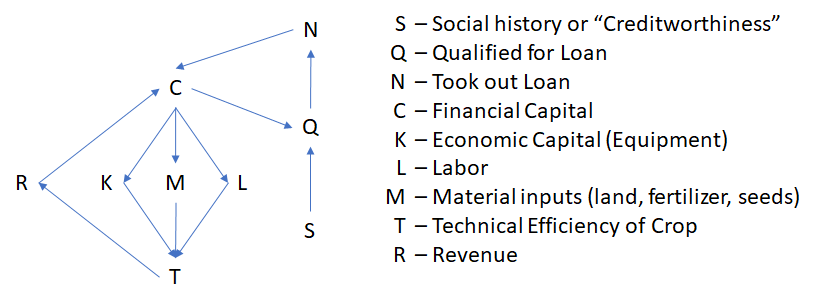
\includegraphics{tables and figures/DAG.png}\\
As I have outlined, the ability for individual i to qualify for a loan
they typically need to have established financial capital and some
measure of trustworthiness to allow for the issuing authority to be
confident that they will recuperate their funds. Financial capital can
be increased by taking a loan, and financial capital is used to purchase
economic capital in the form of durable goods (tools, equipment, etc.),
purchase the raw inputs for the crop (land, fertilizer, seeds, etc.),
and pay for additional labor costs. These factors all then influence the
technical efficiency of the crop, which itself then leads to the
revenues a farmer can expect to receive. These revenues are added back
into the farmer's financial capital, which itself is part of the base
used to establish loan eligibility. Thus, we see that in the system I
have outlined that since revenue is determined by technical efficiency
and influences the ability for a farmer to qualify for a loan there
exists a confounding element within our model.

However, if the loan program the farmers were utilizing in this data was
a special program that did \emph{not} consider other financial elements
when making a decision on credit then the estimate derived might in fact
be a good representation of the desired relationship. However, with the
limited information regarding situation specifics available, the
assumptions made are assumed to be valid.\\

\hfill\break

\hfill\break

\end{document}
